\section{应用方案}
为了满足实时查询的需求,服务需要高性能的PIR协议作为基础。而区块链技术则很好地满足了服务对高可用性的需求。针对黑名单匹配的问题,本文提出了一套向服务提供者委托计算的解决方案。在这一方案中,数据库所有者与服务提供者达成协议,将数据库分片置于服务提供者处。服务提供者通过智能合约处理客户端的在线请求,并通过智能合约不可篡改的属性证明其完成了与数据库所有者之间的协议。这一解决方案保护了客户端的隐私,并确保了客户端、服务提供者和数据库所有者三方的利益。该解决方案的基础采用了第\ref{sec:construction}节中介绍的PIR协议,从而实现了高效的查询处理。
\subsection{协议流程}

\begin{figure}
    \centering
    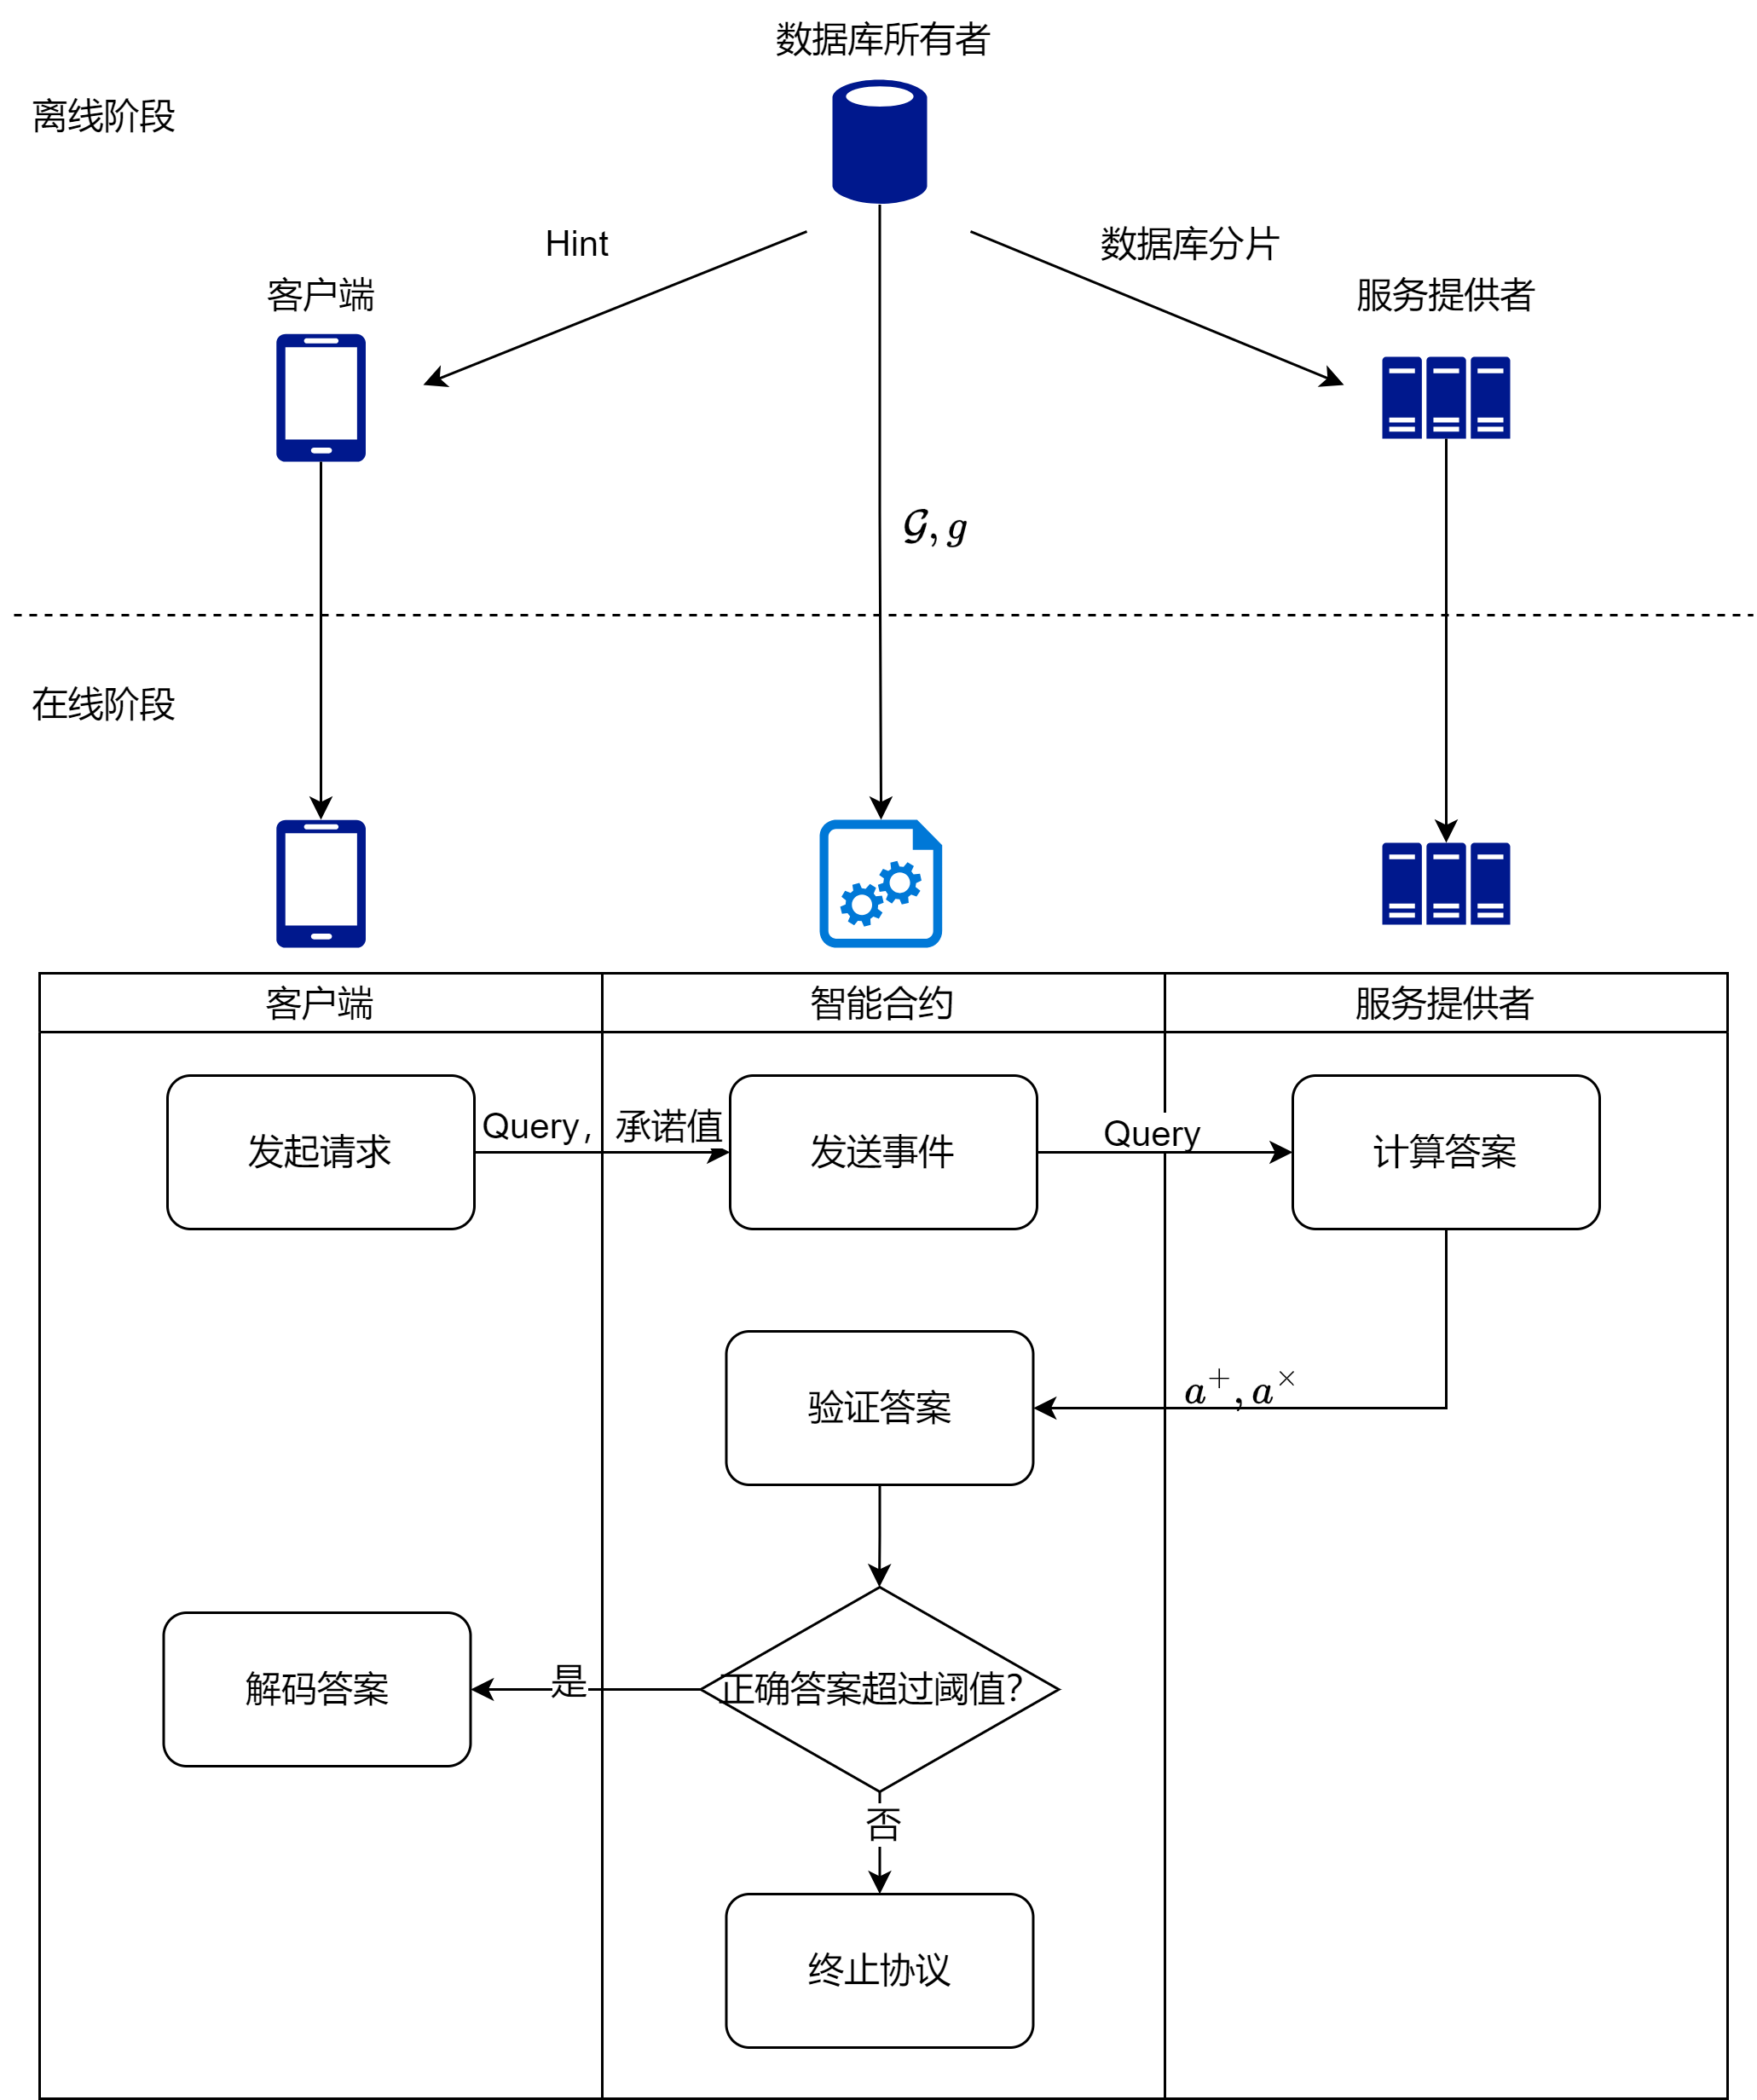
\includegraphics[width=0.8\textwidth]{figure/应用示意图.png}
    \caption{应用示意图}
    \label{fig:pir-application-lane}
\end{figure}

整体应用执行流程如图\ref{fig:pir-application-lane}所示。PIR协议和数据库分片的部分已在第\ref{sec:construction}和第\ref{sec:pir-framework}节中介绍。本节重点关注在线阶段的算法逻辑。算法流程的关键在于确保以下几点:
\begin{enumerate}
    \item 只有当服务提供者提供正确答案时,验证通过。
    \item 只有当通过验证的服务提供者数量超过恢复阈值时,客户端才接受答案。
    \item 若服务提供者未及时响应,则应判定提供的答案无效。如果客户端未及时响应,则视为客户端接受了答案。
\end{enumerate}

这些要求都可以通过智能合约来实现。我们使用Solidity语言编写了相关逻辑,其核心在于验证答案可公开进行。具体来说,协议参与方事先商定一种数据承诺协议,以及一个难解离散对数问题的群$\mathcal{G}$及其生成元$g$:
\begin{enumerate}
    \item 记节\ref{fig:single-server}算法中$Eval(\randomset_\hintidx, \blockidx)$的值为$e$,客户端将$e$承诺至交易中。同时,客户端还将相应的请求与$g^{\randomhint_\hintidx+r\cdot \crumbvalue_{\blockidx, \crumbidx}-e(\sumhint_\hintidx+\crumbvalue_{\blockidx, \crumbidx})}$的值上传至合约内。
    \item 服务提供者提交$\sumanswer,\randomanswer$
    \item 客户端公开$g^e$的值,并验证是否有$g^{\randomhint_\hintidx+r\cdot \crumbvalue_{\blockidx, \crumbidx}-e(\sumhint_\hintidx+\crumbvalue_{\blockidx, \crumbidx})}=g^{\randomanswer-e\sumanswer}$
\end{enumerate}

这一过程中最后验证的等式为
$$g^{\randomhint_\hintidx+r\cdot \crumbvalue_{\blockidx, \crumbidx}-e(\sumhint_\hintidx+\crumbvalue_{\blockidx, \crumbidx})}=g^{\randomanswer-e\sumanswer}$$
对其进行一定的化简,可以得到如下形式:
$$\randomhint_\hintidx+r\cdot \crumbvalue_{\blockidx, \crumbidx}-\randomanswer=e(\sumhint_\hintidx+\crumbvalue_{\blockidx, \crumbidx}-\sumanswer)$$
这个形式与节\ref{fig:single-server}中算法的最终验证等式是一致的。由于群$g$上离散对数问题的困难性,参与方无法从$g^{\randomhint_\hintidx+r\cdot \crumbvalue_{\blockidx, \crumbidx}-e(\sumhint_\hintidx+\crumbvalue_{\blockidx, \crumbidx})}$中恢复出$\randomhint_\hintidx$和$\sumhint_\hintidx$的值。智能合约的具体代码请参见附录\ref{appendix:contract}。具体协议如图\ref{fig:blockchain-scheme}所示。

\begin{figure}
    \begin{mdframed}
        \centering
        \textbf{基于区块链的PIR协议}

        \raggedright
        \textbf{离线阶段:}
        \begin{itemize}
            \item 数据库所有者选择将数据库摘要在链上公开,服务提供者向数据库所有者请求参与协议。根据数据库大小和容灾需要,数据库所有者选择合适的纠删码方案,并在预处理阶段(参见图\ref{fig:framework-protocol})中将数据库分片在链下分发至服务提供者。
            \item 数据库所有者选定离散对数困难的群$\mathcal{G}$及其生成元$g$,并部署相应的智能合约。
            \item 客户端与数据库所有者在链下运行PIR协议的离线阶段,以获取所需的Hint和Crumb。
        \end{itemize}
        \textbf{在线阶段:}
        \begin{itemize}
            \item 客户端通过智能合约发起交易,并执行PIR协议的$Query$算法,将承诺值和请求上传至合约,触发交易事件。
            \item 服务提供者检测到交易并计算查询结果,执行PIR协议的$Answer$算法,将答案上传至智能合约。
            \item 智能合约验证答案的正确性,若通过解码阈值的验证,则客户端解码并接受答案;若未通过,则客户端拒绝答案并结束协议。
        \end{itemize}
    \end{mdframed}
    \caption{基于区块链的PIR协议}
    \label{fig:blockchain-scheme}
\end{figure}

对客户端和服务提供者而言,其交互逻辑与第\ref{sec:pir-framework}节中PIR框架的运行基本一致。唯一的区别在于双方不再直接进行交互,而是通过智能合约进行中转。双方的通信均被记录在智能合约上。正如前文所述,这些通信记录起到了数据库所有者与服务提供者之间的信用证明作用。由于客户端的计算量较小,常见的个人设备都能胜任,因此该方案可以轻松移植至移动设备、浏览器等环境中。

\begin{figure}
    \centering
    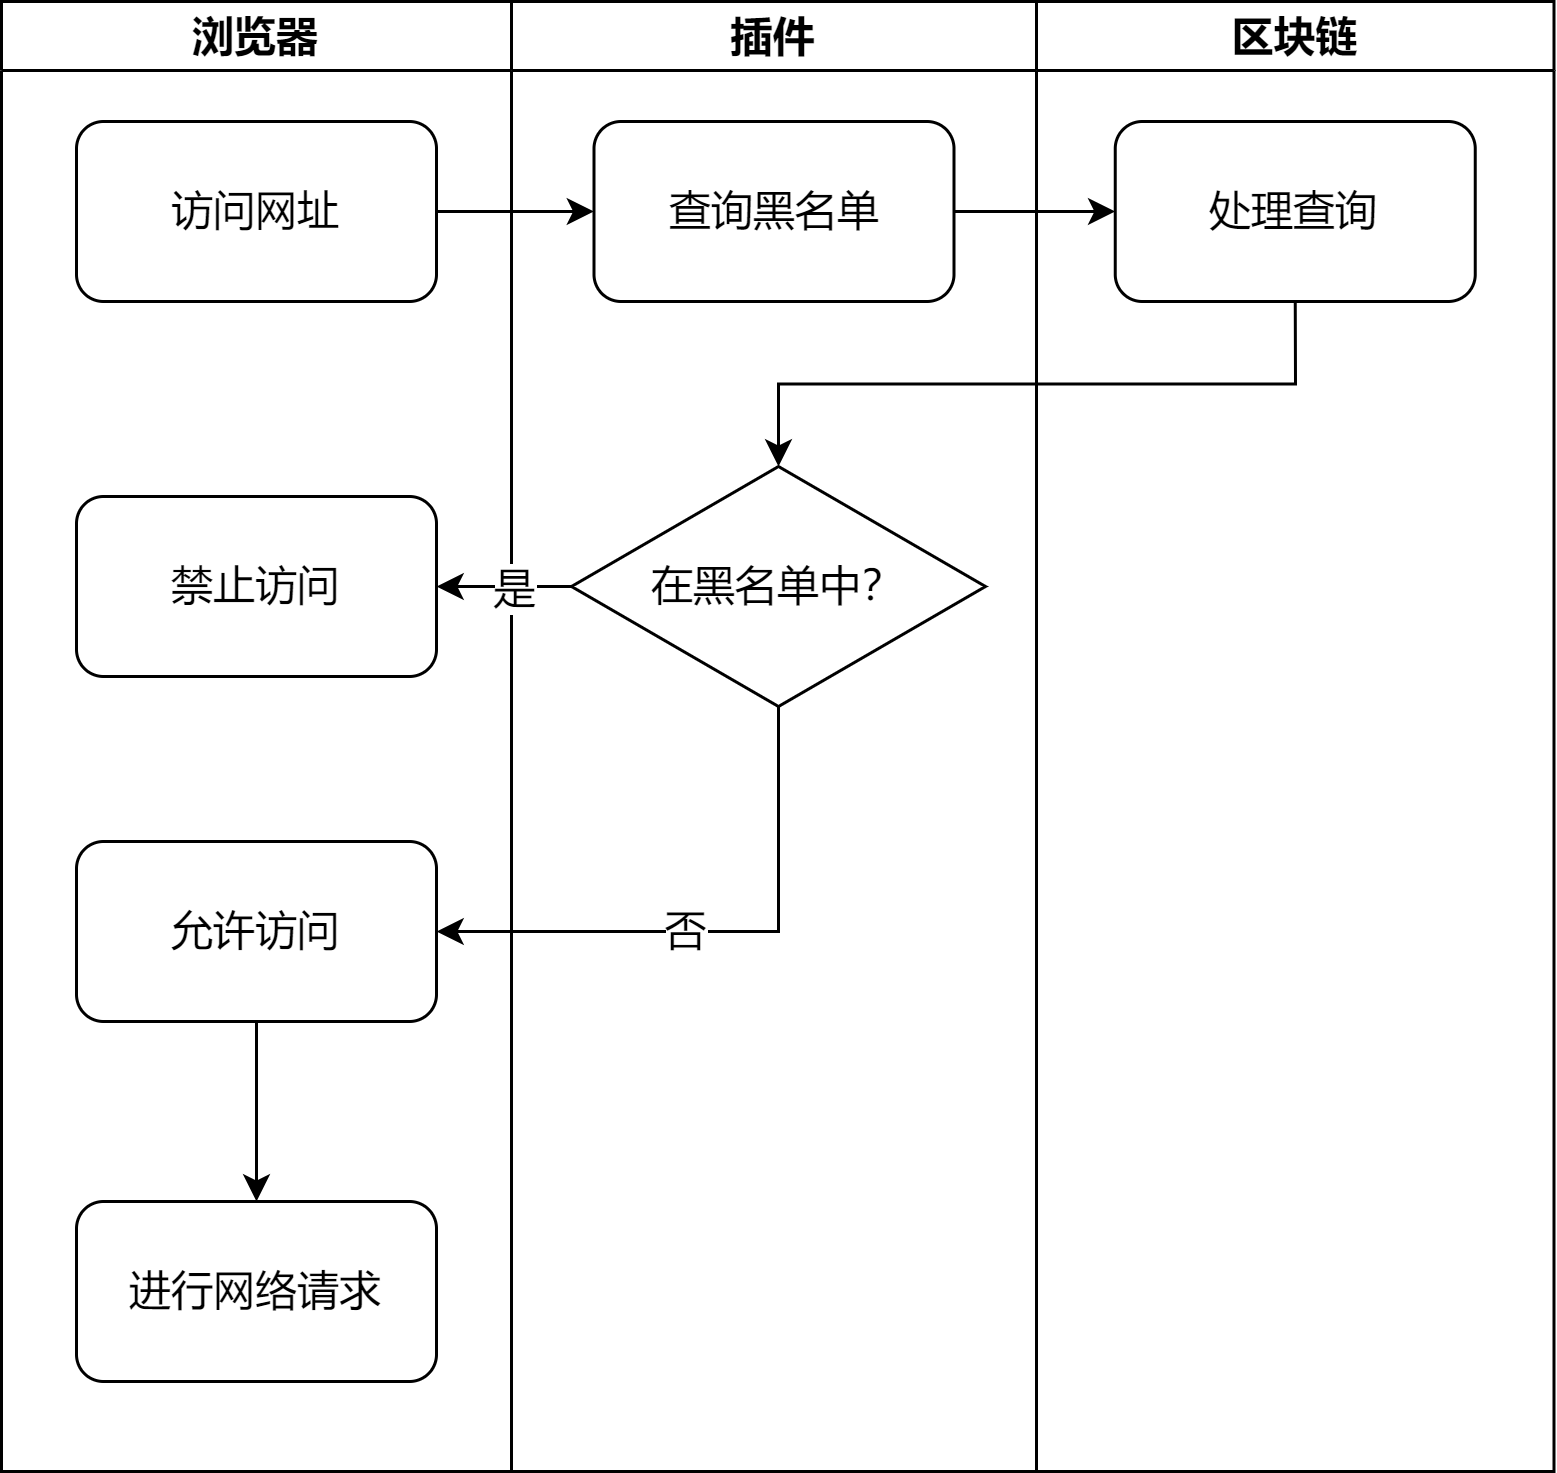
\includegraphics[width=0.8\textwidth]{figure/浏览器逻辑.png}
    \caption{网址黑名单查询服务流程}
    \label{fig:pir-application-browser}
\end{figure}


\begin{figure}
    \centering
    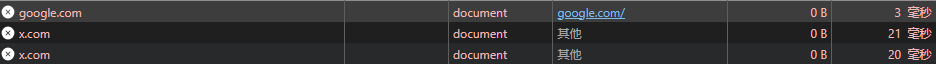
\includegraphics[width=0.8\textwidth]{figure/blocking_requests.png}
    \caption{被阻止的网络请求}
    \label{fig:blocking-requests}
\end{figure}
实践中,我们将这一查询服务集成至浏览器内,为用户提供诈骗网站预警服务。如图\ref{fig:pir-application-browser}所示,服务以插件形式拦截浏览器请求,将相应的域名提交至智能合约查询。如图\ref{fig:blocking-requests}所示,如果发现访问的域名在黑名单中,插件将阻止相应的网络请求。这一方案兼顾了用户隐私保护与诈骗网址拦截的需求。



\subsection{将关键字PIR转化为标准PIR}
在黑名单查询中,客户端通常要查询的不是由稠密索引定位的记录,而是离散的关键词。因此,协议需要将关键词查询转换为索引查询。相关研究已经相当成熟,例如Checklist\cite{USENIX:KogCor21}采用一种基于哈希的方法,将关键词映射为哈希值。该方法首先查询本地映射表,检查是否存在关键词对应的哈希前缀,然后通过PIR查询哈希前缀以获取完整哈希来验证是否命中黑名单。这种方式非常适用于黑名单查询场景:在与黑名单查询相关的服务中,大多数查询结果是阴性的,只有少数查询项属于黑名单。由于采用了前缀-完整哈希的两级查询方式,许多查询可以在客户端本地直接被排除,从而节省大量在线计算和通信成本。本文在本节中直接采用了这种方法,不再深入讨论。